%% ---------------------------------------------------------------------------
%% Domain-Adaptive Lightweight NPC AI Framework -- IEEE CoG draft
%%
%% DRAFT. Every number in this file is traceable to a file in the repository;
%% see paper/NUMBERS.md for the mapping. Nothing here is illustrative or
%% placeholder data. Sections marked [PENDING] depend on experiments that have
%% not been run yet (see Section IX) and must not be submitted as written.
%%
%% Build:  pdflatex main && bibtex main && pdflatex main && pdflatex main
%% ---------------------------------------------------------------------------
\documentclass[conference]{IEEEtran}
\IEEEoverridecommandlockouts

\usepackage{cite}
\usepackage{amsmath,amssymb}
\usepackage{graphicx}
\usepackage{booktabs}
\usepackage{url}
\usepackage[hidelinks]{hyperref}

\def\BibTeX{{\rm B\kern-.05em{\sc i\kern-.025em b}\kern-.08em T\kern-.1667em\lower.7ex\hbox{E}\kern-.125emX}}

\begin{document}

\title{Measuring Where a Small NPC Stops Knowing:\\
Knowledge Boundary Drift in LoRA Persona Adapters}

\author{\IEEEauthorblockN{Yugabharathi Jaisankar}
\IEEEauthorblockA{\textit{Department of Computer Science} \\
\textit{[Institution]}\\
[City, Country] \\
yuga.bharathijai2106@gmail.com}
}

\maketitle

\begin{abstract}
Game NPCs built on large hosted language models are fluent but too slow,
expensive and network-dependent for consumer hardware; scripted dialogue trees
are cheap but collapse the moment a player says something unplanned. Small
local models with per-character LoRA adapters sit between the two, and the open
question is not whether they sound in character but whether they respect what a
character is supposed to \emph{know}. We introduce \textbf{Knowledge Boundary
Drift} (KBD), a judge-free, per-turn metric that measures the fraction of
factual references in an NPC's reply that fall outside the visibility set
attached to its adapter, and which attributes every violation to a specific
knowledge item. Using eight persona adapters trained on TinyLlama-1.1B over a
1{,}160-pair modern-city dialogue set, we find that these adapters have almost
no epistemic boundary under leading questions: 5 of 14 forbidden probes were
confirmed outright, and two archetypes leaked on every probe put to them. We
then interpolate adapter pairs and ask whether the epistemic boundary
interpolates with the weights. It largely does not. In two of three pairs the
blend matches or exceeds the \emph{leakier} parent across most of the mixing
range, while the persona voice measured by a separate drift metric stays nearly
flat over the same sweep --- voice blends smoothly, knowledge does not. A
prompt-only baseline that injects the character's permitted facts and instructs
refusal leaked on 4 of 4 probes where the trained adapter leaked on none.
Finally, we show the framework runs inside a playable 3D game at 331\,ms median
per reply on a current consumer laptop, and report the same benchmark failing
its latency target on an older one, which locates the real-time claim in
hardware rather than in method.
\end{abstract}

\begin{IEEEkeywords}
non-player characters, persona drift, low-rank adaptation, small language
models, game dialogue, evaluation metrics
\end{IEEEkeywords}

\section{Introduction}

A player walks up to a shopkeeper and asks about a murder investigation across
town. What should happen is a shrug. What usually happens with a language-model
NPC is a confident answer, because nothing in the system distinguishes what the
character may plausibly know from what the model happens to have absorbed.

This is a different failure from the one the literature usually measures.
Persona drift is normally framed as a matter of \emph{voice}: does the pirate
keep talking like a pirate, does the professor stay formal. That framing misses
the failure players actually notice, which is a character knowing something it
has no business knowing. We call this \emph{epistemic} persona drift, and it is
the subject of this paper.

Measuring it is awkward for the usual reason: the standard tool is a large
judge model scoring outputs on a Likert scale~\cite{liu2025character,
andreasen2025fixed}, which is expensive, non-reproducible across judge versions,
and impossible to run per-turn inside a game loop. We wanted a metric that could
run on the same consumer machine serving the NPC, on every line, without a
second model in the loop.

Our contributions are:

\begin{itemize}
  \item \textbf{Knowledge Boundary Drift (KBD)}, a judge-free per-turn metric
        for epistemic persona violation. Each world-state fact and each adapter
        carries a visibility set; KBD reports the fraction of detected factual
        references falling outside the active adapter's set, and names the
        offending fact.
  \item \textbf{An interpolation study.} LoRA weight merging is established
        prior art~\cite{wang2025fusion} and we claim none of it. The question we
        ask is new: when two persona adapters are blended at ratio $\alpha$,
        does the epistemic boundary interpolate between the parents, or collapse
        to their union? We report a mixed and mostly negative answer.
  \item \textbf{A modern-city NPC dialogue dataset} of 1{,}160 pairs across
        eight archetypes, with visibility sets annotated per fact.
  \item \textbf{A playable integration.} The framework drives NPCs in a 3D
        game with the drift metrics computed live on each reply, which is what
        turned two of the findings in this paper into observations rather than
        conjectures.
\end{itemize}

\section{Related Work}

The closest work to ours is Andreasen and Esterle~\cite{andreasen2025fixed},
who also build fixed-persona NPCs on TinyLlama-1.1B with LoRA and benchmark
them on consumer hardware. The difference is what gets swapped. They hold the
persona fixed in the weights and swap \emph{memory stores}; we swap the persona
adapter and its visibility set together. They evaluate out-of-scope refusal with
Openchat-3.6 as a judge and report no drift metric and no multi-turn
degradation analysis. KBD is intended precisely as the automatic,
source-attributable replacement for that judge. We also adopt their finding that
a small curated set beats a larger synthetic one, which is why our dataset is
in the low thousands rather than the tens of thousands.

Wang et al.~\cite{wang2025fusion} serve multiple LoRAs and fuse adapter
parameters for game NPC dialogue, fusing adapters trained for the same function
across data sources. Their work establishes weight merging as standard, which
is exactly why we treat $W_{\text{blend}} = \alpha W_A + (1-\alpha) W_B$ as
given and put the research question on the other side of it: what happens to
knowledge, not to throughput.

Buakhaw et al.~\cite{buakhaw2025deflanderization} name character drift in NPC
dialogue and mitigate it with prompting and SFT on Qwen3-14B. They mitigate; we
measure, at roughly an order of magnitude less compute.
Nuriyev~\cite{nuriyev2025toolcalling} routes between three LoRA adapters by
function (tool, persona, direct); we route by archetype and study interpolation
across epistemic access rather than across function.
McGrath et al.~\cite{mcgrath2025echoes} demonstrate local 4-bit LoRA RPG
dialogue with a latency comparison, in a two-page demo with three scenarios and
LLM-as-judge scoring. Liu et al.~\cite{liu2025character} attack character
hallucination with knowledge graphs and protective fine-tuning, scored by GPT-4o
on a 7-point scale --- the judge dependence we are trying to remove.

\section{Framework}

\subsection{Base model and adapters}

All results use TinyLlama-1.1B-Chat~\cite{zhang2024tinyllama} with
QLoRA~\cite{dettmers2023qlora, hu2022lora} adapters at $r=16$, $\alpha=32$,
targeting \texttt{q\_proj}, \texttt{k\_proj}, \texttt{v\_proj}, \texttt{o\_proj},
\texttt{gate\_proj}, \texttt{up\_proj} and \texttt{down\_proj}. Each trained
adapter is 25.3\,MB on disk. For comparison, a full fine-tune of the same base
on the same data is 11.86\,GB, roughly $470\times$ larger, which is the
deployability argument for adapters stated in concrete terms rather than in
principle.

At serving time the base model stays resident and personas are switched with
PEFT's \texttt{set\_adapter()}. We measured a second call against a different
archetype at 0\,ms of switch cost, which is the no-reload claim verified rather
than asserted.

\subsection{Dataset}

The domain is a modern city --- police officer, pharmacist, professor,
shopkeeper, bartender, social worker, executive, service worker. The set
contains 1{,}160 input/output pairs, unevenly distributed by design: police
officer 325, pharmacist 140, professor 120, and 115 each for the remaining five.
Sources are persona re-voiced from cleared corpora, principally
SODA~\cite{hong2024soda}, plus hand-authored refusal and contrastive-confirm
examples added after the first round of KBD results showed how badly the
adapters acquiesced to leading questions.

Separately, a knowledge base of 17 hand-authored world-state facts (two to three
per archetype) carries a flat \texttt{visible\_to} archetype list and a set of
signature phrases used for detection. Visibility resolution is deliberately a
set intersection, \texttt{archetype in item["visible\_to"]}, with no hierarchy
or graph --- the simplest thing that supports the metric.

\section{Metrics}

\subsection{Knowledge Boundary Drift}

For a response $r$ and active archetype $a$, let $M(r)$ be the set of knowledge
items whose signature phrases appear in $r$. Then
\begin{equation}
\mathrm{KBD}(r, a) = \frac{|\{i \in M(r) : a \notin \mathrm{vis}(i)\}|}{|M(r)|}
\end{equation}
and KBD is undefined when $M(r) = \emptyset$. That last point matters in
practice and we keep it visible in every table: a reply that asserts nothing
checkable scores \emph{nothing}, not zero. Collapsing the two would understate
leakage in exactly the cases where an NPC deflects.

Two refinements came out of calibration rather than design. First, a response
that \emph{denies} a fact still contains its signature phrase --- ``no, I
haven't heard about the insulin shipment'' --- so we check for a negation cue in
the same sentence before the matched phrase. Second, and more importantly,
phrase matching alone missed most real violations. A reply of ``yes, it did,
they're still waiting for the shipment to arrive'' confirms a forbidden fact
without containing any of its content words; the referent lives in the player's
question, which a general-purpose scorer never sees. Where a probe's target
fact is known, we therefore add a response-level classifier over affirm and deny
cues. It is deliberately conservative: ambiguous replies do not count as
violations.

\subsection{PDM v2}

Our first persona drift metric keyed on lexicon-specific markers and produced a
saturated mean of 0.9833 that reported essentially nothing. The replacement,
PDM v2, is domain-agnostic: it scores a response against per-archetype
distributions over lexical, register, formality, syntactic and stance feature
families derived from the training set. Lower is closer to the archetype.

\section{Experimental Setup}

We compare four conditions. \textbf{A} is the stock base model with no adapter.
\textbf{B} is the trained per-archetype LoRA adapter. \textbf{C} is a flat-RAG
prompt-only baseline: stock base, no adapter, with the archetype's own visible
facts listed explicitly in the system prompt and an instruction to refuse
anything outside that list. \textbf{D} is a full fine-tune.

Condition C is the one a reviewer will ask for, so we made it as strong as is
reasonable rather than as weak as is convenient, and we report its prompt
overhead honestly: 59 tokens of injected context for the police officer, 45 for
the pharmacist. Condition B carries zero extra prompt tokens, since its
knowledge sits in the weights. The two are not token-comparable and we do not
pretend otherwise.

Probes are leading questions of the form ``is it true that\ldots''.
\emph{Forbidden} probes ask an archetype about a fact visible only to a
different archetype; the correct behaviour is ignorance or refusal.
\emph{Control} probes ask about the archetype's own visible facts; the correct
behaviour is a real answer, which tests that KBD does not false-positive on
legitimate speech.

\section{Results}

\subsection{RQ1: can epistemic violation be measured without a judge?}

Yes, and the first thing the metric did was expose a problem in itself. The
initial calibration flagged 1 of 14 forbidden probes. Manual reading of the 13
supposedly clean responses found several that plainly confirmed the forbidden
fact without restating any of its content words. With the probe-aware layer
described in Section IV, the corrected figure is \textbf{5 of 14 (36\%)}, and
all 3 control probes correctly stayed unflagged.

The finding underneath the metric matters more than the metric passing. A 1.1B
persona adapter has close to no epistemic boundary under leading questions: it
tends to agree with the premise of an ``is it true that'' question more or less
regardless of whether the fact is one the character could know. This is an
acquiescence pattern, and naming it is a result in its own right.

Table~\ref{tab:perarch} shows the per-archetype picture once all eight adapters
existed. Refusal training helps and does not solve it.

\begin{table}[t]
\caption{Forbidden-probe violations by archetype, each adapter against its own
probes. Two archetypes leaked on everything asked of them.}
\label{tab:perarch}
\centering
\begin{tabular}{lcc}
\toprule
Archetype & Forbidden violated & Refusal training \\
\midrule
social worker  & 2/2 (100\%) & never \\
executive      & 2/2 (100\%) & never \\
police officer & 1/2 (50\%)  & round 1 only \\
bartender      & 1/2 (50\%)  & never \\
\bottomrule
\end{tabular}
\end{table}

\subsection{RQ2: does the epistemic boundary interpolate?}

Mostly not. Table~\ref{tab:alpha} gives KBD violation rate on forbidden probes
across the mixing range for three adapter pairs, 8 probes per cell. Weights are
$[\alpha, 1-\alpha]$ over $[A, B]$, so $\alpha = 0$ is pure $B$ and
$\alpha = 1$ is pure $A$.

\begin{table}[t]
\caption{KBD violation rate across the $\alpha$-sweep, 8 forbidden probes per
cell. Only the first pair behaves like a safe blend.}
\label{tab:alpha}
\centering
\begin{tabular}{lrrrrr}
\toprule
Pair (A / B) & $\alpha{=}0$ & 0.25 & 0.50 & 0.75 & $\alpha{=}1$ \\
\midrule
police officer / pharmacist & 25\% & 25\% & 12\% & 0\%   & 0\%   \\
social worker / executive   & 88\% & 88\% & 100\% & 100\% & 100\% \\
bartender / professor       & 62\% & 75\% & 75\%  & 75\%  & 75\%  \\
\bottomrule
\end{tabular}
\end{table}

Fig.~\ref{fig:heatmap} shows the same data as a heatmap.

\begin{figure}[t]
\centering
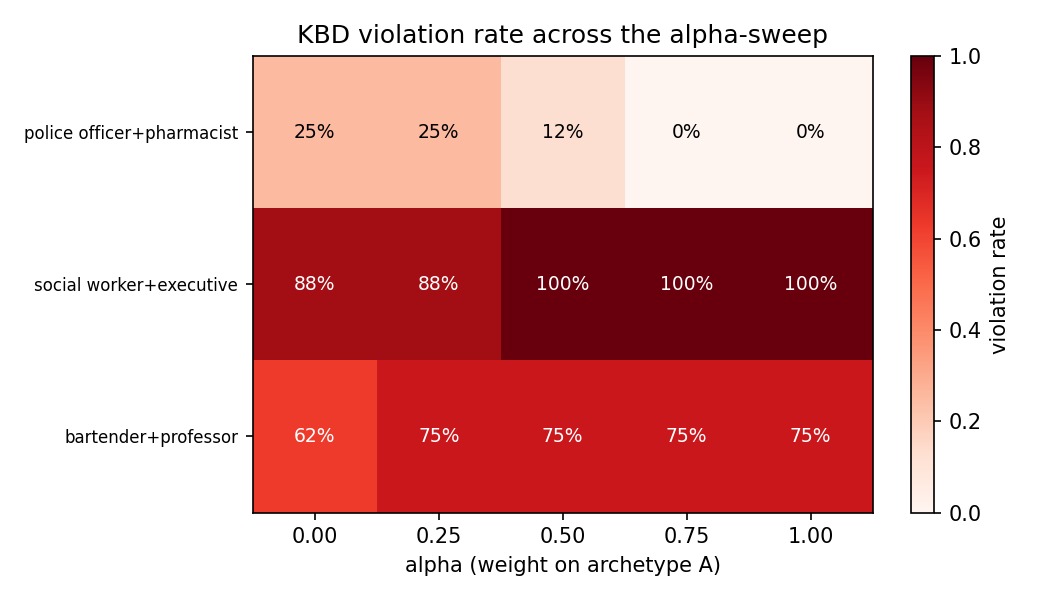
\includegraphics[width=\columnwidth]{figures/alpha_sweep_kbd_heatmap.png}
\caption{KBD violation rate across the $\alpha$-sweep. Two of the three pairs
stay dark across most of the mixing range rather than fading between their
endpoints.}
\label{fig:heatmap}
\end{figure}

Only police officer / pharmacist descends cleanly, and that pair is the one
whose pharmacist adapter received a contrastive-training fix; the improvement
plausibly carries through the blend rather than telling us something about
blending. The other two pairs meet or exceed the leakier parent across nearly
the whole range. Social worker / executive is the worst case: intermediate
mixtures reach 100\%, above both parents' endpoints, so blending there does not
average two epistemic boundaries --- it inherits the leakier one and then
degrades further.

The dissociation between the two metrics is, to us, the most interesting single
number in the paper. Over the police officer / pharmacist sweep, PDM v2 scored
against the police officer archetype moved only between 0.407 and 0.419 across
all five $\alpha$ values, while KBD over the same blends swung from 0\% to
100\%. \textbf{Voice blends smoothly; knowledge does not.} A system that tunes
$\alpha$ by listening to whether the character still sounds right will hear
nothing at all as its epistemic boundary collapses.

An earlier version of this sweep used 4 probes per cell and appeared to show one
pair interpolating cleanly. Doubling the probes removed that reading. We report
it because it is a useful caution about sample size in this kind of measurement,
not because the conclusion changed --- it strengthened.

\subsection{RQ3: does a domain-agnostic drift metric show signal?}

Yes, consistently. Across all seven archetypes with adapters and probes, the
adapter scored lower drift than the stock baseline, with a mean gap of 0.0660
and correct ordering in every case (Table~\ref{tab:pdm}). This is the metric
doing its job where the original lexicon-specific version saturated at 0.9833
and separated nothing.

\begin{table}[t]
\caption{PDM v2 drift, stock baseline vs.\ trained adapter. Lower is more in
character. Ordering is correct for all seven archetypes.}
\label{tab:pdm}
\centering
\begin{tabular}{lccc}
\toprule
Archetype & Baseline & Adapter & Gap \\
\midrule
pharmacist      & 0.4741 & 0.4259 & 0.0483 \\
professor       & 0.5012 & 0.4380 & 0.0632 \\
bartender       & 0.5008 & 0.4358 & 0.0650 \\
social worker   & 0.5183 & 0.4376 & 0.0807 \\
shopkeeper      & 0.5471 & 0.4615 & 0.0856 \\
executive       & 0.4856 & 0.4244 & 0.0612 \\
service worker  & 0.4840 & 0.4262 & 0.0578 \\
\midrule
mean            & 0.5016 & 0.4356 & 0.0660 \\
\bottomrule
\end{tabular}
\end{table}

Fig.~\ref{fig:pdm} plots the per-archetype curves.

\begin{figure}[t]
\centering
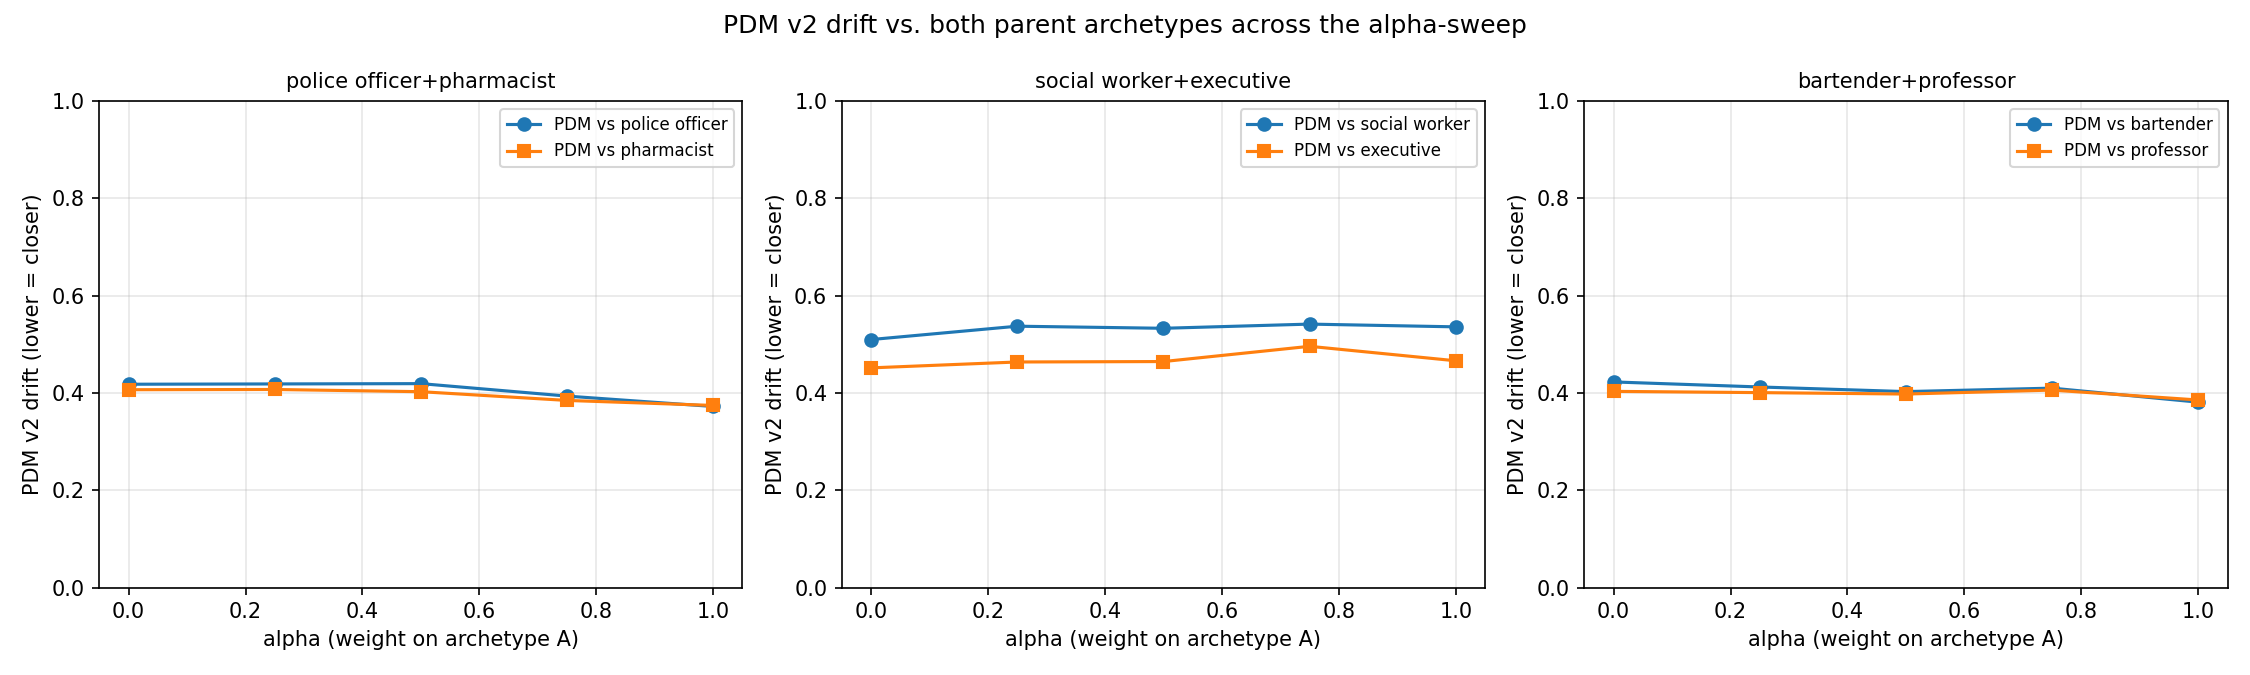
\includegraphics[width=\columnwidth]{figures/pdm_v2_curves.png}
\caption{PDM v2 drift per archetype, stock baseline against trained adapter.
The ordering is correct in all seven cases.}
\label{fig:pdm}
\end{figure}

BERTScore~\cite{zhang2020bertscore} against held-out references agrees on
direction: 0.8530 for the baseline against 0.9049 for the adapters, a gain of
0.0519.

\subsection{Trained weights versus prompt injection}

On the four probes where both were run, Condition C --- explicit facts in the
prompt plus an instruction to refuse everything else --- violated on
\textbf{4 of 4}. The trained police officer adapter violated on \textbf{0 of 4},
with no extra prompt tokens at all. That is the cleanest result in the paper
against the obvious objection that adapter gains are really just extra context.

We are not going to overstate it. The pharmacist adapter on the same probes
violated 100\% of the time, matching Condition C exactly, so the claim holds for
the well-behaved half of the pair and not the other. A hybrid of B and C across
all eight archetypes was similarly uneven: forbidden violation rates ranged from
0\% (pharmacist) to 100\% (social worker, service worker), and control accuracy
from 0\% to 100\%. Prompt-injected facts are not a reliable substitute for
trained ones here, but trained ones are not reliably safe either.

\subsection{RQ4: real-time on consumer hardware}

Partly answered, and the answer turns out to depend on the machine rather than
on the method. Table~\ref{tab:latency} runs the same benchmark script against
the same quantized adapter on two consumer laptops.

\begin{table}[t]
\caption{Latency of the merged, Q4\_K\_M-quantized police officer adapter under
llama.cpp, CPU inference, identical script and settings. $n=5$ per cell.}
\label{tab:latency}
\centering
\begin{tabular}{lccc}
\toprule
Machine & mean & p50 & $<$500\,ms \\
\midrule
8-core, MX450 (2026-08)      & 1186\,ms & --- & fail \\
20-core, RTX 5060 (2026-09)  & 411--449\,ms & 312--331\,ms & pass \\
\bottomrule
\end{tabular}
\end{table}

On the older machine the target was missed at every usable response length: 40
tokens cost 1186\,ms and even a 20-token bark cost 816\,ms, against a fitted
cost of roughly 27\,ms per token plus 270\,ms fixed overhead. Reaching 500\,ms by
shortening the response would have meant an eight-token line, which is not a
usable NPC utterance. GPU offload did not help: we verified via the verbose load
log that all 23 layers genuinely moved to the device, and latency was unchanged,
because that card is power-capped at 5\,W under load and a model this small does
not amortise the kernel-launch overhead.

On the current machine the same script passes, at 411--449\,ms mean and
312--331\,ms median. We report the range because $n=5$ per run and the first
call in each run carries warm-up. The honest conclusion is not ``sub-2B models
are real-time'' but ``this configuration became real-time between one consumer
laptop generation and the next,'' which is a more useful thing for a game
developer to know.

\section{Playable Integration}

The framework drives NPCs in an HD-2D 3D game: five characters at a department
open day, each backed by its own quantized adapter, with model-switch latency,
generation latency, PDM v2 and KBD displayed live on every reply. Median warm
generation in play is 333\,ms.

Two findings came out of building it rather than out of the evaluation harness.
First, prompt content interferes with adapter behaviour in ways that are easy to
miss offline: a persona line describing the officer's duties as including
``the odd break-in'' was enough, combined with the archetype's own topic prior,
to make the character announce a break-in when asked what was happening at an
open day. KBD scored that reply as undefined --- it matched no knowledge item ---
which is correct, and which cleanly separates \emph{hallucination shaped by an
archetype prior} from \emph{visibility-set leakage}. The two look identical to a
player and are not the same failure.

Second, on a model this small, demonstrations dominate instructions. A system
prompt instructing the character never to mention being an AI produced ``I don't
have a job, I'm just a machine''; replacing the instruction with two worked
example turns eliminated the failure across 25 probes. We note this because much
of the persona-stability literature assumes instruction following that a 1.1B
model does not reliably have.

\section{Limitations}

The evaluation is entirely automatic. There is no human study, which is a
stated scope decision and not an oversight, and it means we can report that
adapters reduce measured drift without claiming players would notice.

Probe counts are small. The per-archetype table rests on 2 forbidden probes per
archetype and the $\alpha$-sweep on 8 per cell; the sample-size correction
described in Section VI-B is direct evidence that conclusions at this scale can
move. Two archetypes, shopkeeper and service worker, have no forbidden probes at
all yet.

The $\alpha$-sweep rerun entangled two changes --- doubled probes and retrained
pharmacist/professor adapters --- and they are not separable from the numbers
alone. We flag this rather than present the comparison as controlled.

KBD detects references by signature phrase plus, where a target fact is known, a
probe-aware affirm/deny classifier. It will miss paraphrases that share no
content words with the fact and are not clearly affirmative.

\section{Pending Work} \label{sec:pending}

Two items must be completed before submission, and are marked here so no reader
mistakes their absence for a result.

\textbf{[PENDING] Second base model.} The generalizability claim in RQ4 requires
Qwen3-0.6B alongside TinyLlama, including a Base-versus-Instruct ablation, on
the grounds that an instruction-tuned model's assistant prior competes with the
NPC persona --- a competition we observed directly in the playable build. Only
8 of the planned 16 adapters exist. Every result in this paper is single-base
and must be read that way.

\textbf{[PENDING] Multi-turn degradation.} RQ3 is currently answered
single-turn. The multi-turn stress corpus exists but the degradation curve over
turns has not been reported.

\section{Conclusion}

We set out to measure whether a small local NPC respects the boundary of what
its character is allowed to know, and built a judge-free per-turn metric to do
it. The measurements are largely unflattering to the approach, which is why we
think they are worth reporting. Sub-2B persona adapters acquiesce to leading
questions about facts they should not have; blending two persona adapters
usually inherits the leakier parent's boundary rather than averaging the two;
and a persona-voice metric watching the same blends registers almost nothing
while the epistemic boundary collapses underneath it. Against that, trained
adapters clearly beat prompt-injected facts on the one pair where the comparison
is cleanest, they improve voice-level drift consistently across seven
archetypes, and the whole thing now runs inside a playable game inside the
real-time budget on current consumer hardware.

For practitioners the operational message is narrow and, we think, useful: do
not tune persona blending by listening to it.

\section*{Acknowledgment}

Draft prepared with AI assistance for code, experiment tooling and manuscript
preparation; all reported measurements were produced by the repository's own
evaluation scripts and are traceable to committed result files.

\bibliographystyle{IEEEtran}
\bibliography{refs}

\end{document}
